% $Id: jfsample.tex,v 19:a118fd22993e 2013/05/24 04:57:55 stanton $
\documentclass[11pt]{article}

% DEFAULT PACKAGE SETUP

\usepackage{setspace,graphicx,epstopdf,amsmath,amsfonts,amssymb,amsthm}
\usepackage{marginnote,datetime,enumitem,subfigure,rotating,fancyvrb}
\usepackage{hyperref,float}
\usepackage[longnamesfirst]{natbib}
\usdate

% These next lines allow including or excluding different versions of text
% using versionPO.sty

% Notes options
\ifnotes{%
\usepackage[margin=1in,paperwidth=10in,right=2.5in]{geometry}%
\usepackage[textwidth=1.4in,shadow,colorinlistoftodos]{todonotes}%
}{%
\usepackage[margin=1in]{geometry}%
\usepackage[disable]{todonotes}%
}

% Allow todonotes inside footnotes without blowing up LaTeX
% Next command works but now notes can overlap. Instead, we'll define 
% a special footnote note command that performs this redefinition.
%\renewcommand{\marginpar}{\marginnote}%

% Save original definition of \marginpar
\let\oldmarginpar\marginpar

% Workaround for todonotes problem with natbib (To Do list title comes out wrong)
\makeatletter\let\chapter\@undefined\makeatother % Undefine \chapter for todonotes

% Define note commands
\newcommand{\smalltodo}[2][] {\todo[caption={#2}, size=\scriptsize, fancyline, #1] {\begin{spacing}{.5}#2\end{spacing}}}
\newcommand{\rhs}[2][]{\smalltodo[color=green!30,#1]{{\bf RS:} #2}}
\newcommand{\rhsnolist}[2][]{\smalltodo[nolist,color=green!30,#1]{{\bf RS:} #2}}
\newcommand{\rhsfn}[2][]{%  To be used in footnotes (and in floats)
\renewcommand{\marginpar}{\marginnote}%
\smalltodo[color=green!30,#1]{{\bf RS:} #2}%
\renewcommand{\marginpar}{\oldmarginpar}}
%\newcommand{\textnote}[1]{\ifnotes{{\noindent\color{red}#1}}{}}
\newcommand{\textnote}[1]{\ifnotes{{\colorbox{yellow}{{\color{red}#1}}}}{}}

% Command to start a new page, starting on odd-numbered page if twoside option 
% is selected above
\newcommand{\clearRHS}{\clearpage\thispagestyle{empty}\cleardoublepage\thispagestyle{plain}}

% Number paragraphs and subparagraphs and include them in TOC
\setcounter{tocdepth}{2}

% JF-specific includes:

\usepackage{indentfirst} % Indent first sentence of a new section.
\usepackage{endnotes}    % Use endnotes instead of footnotes
\usepackage{jf}          % JF-specific formatting of sections, etc.
\usepackage[labelfont=bf,labelsep=period]{caption}   % Format figure captions
\captionsetup[table]{labelsep=none}

% Define theorem-like commands and a few random function names.
\newtheorem{condition}{CONDITION}
\newtheorem{corollary}{COROLLARY}
\newtheorem{proposition}{PROPOSITION}
\newtheorem{obs}{OBSERVATION}
\newcommand{\argmax}{\mathop{\rm arg\,max}}
\newcommand{\sign}{\mathop{\rm sign}}
\newcommand{\defeq}{\stackrel{\rm def}{=}}

\begin{document}

\setlist{noitemsep}  % Reduce space between list items (itemize, enumerate, etc.)
\onehalfspacing      % Use 1.5 spacing
% Use endnotes instead of footnotes - redefine \footnote command
\renewcommand{\footnote}{\endnote}  % Endnotes instead of footnotes

\author{RICHARD STANTON\thanks{\rm Stanton is with the Haas
      School of Business, U.C. Berkeley. Acknowledgments \ldots}}

\title{\Large \bf A Sample JF Paper}

\date{}              % No date for final submission

% Create title page with no page number

\maketitle
\thispagestyle{empty}

\bigskip

\centerline{\bf ABSTRACT}

\begin{doublespace}  % Double-space the abstract and don't indent it
  \noindent There's nothing very interesting here, but the format (achieved using the file \texttt{jf.sty}) makes it suitable for publication in the \emph{Journal of Finance} even if the content doesn't. Here's a nice, informative, double-spaced abstract.
\end{doublespace}

\medskip

\noindent JEL classification: XXX, YYY.

\clearpage


\noindent Note that the JF doesn't want the first section to be titled, and the text here is not indented.\footnote{Here's a sample footnote (endnote).} Let's put in some sections and subsections to see how they get formatted.

\section{The Model} \label{sec:Model}

There's not actually a model here as it's not really a paper, but this is about where a model might go. Note that the first sentence of this section is indented (as required by the JF) using the \texttt{indentfirst} package.

\subsection{A Subsection}

Note that subsections in JF are just labeled with letters.  When referring to them in the text, you need to add the section number back, e.g., Section~\ref{sec:subsec} or~\ref{sec:subsub}. This is taken care of in \texttt{jf.sty}. Let's also add some parenthetical citations (see~\cite{Stanton:95}, \cite{CarpenterStantonWallace:12}, \cite{Campbell:03}). 

To justify adding a subsection here, from now on, we'll assume
\begin{condition}\label{cond:rates}
$0 <  \hat{\mu} < \gamma\sigma^2$.
\vspace{3mm}
\end{condition}
This condition might be useful if there was a model. 

\subsection{Another Subsection, With a Figure}
\label{sec:subsec}

Figures get put at the end, with a note marking where they should go in the text, like this:

\bigskip
\centerline{\bf [Place Figure~\ref{fig:0} about here]}
\bigskip

\subsubsection{A Subsubsection with a Proposition}
\label{sec:subsub}

Let's put a proposition here.
\begin{proposition} \label{prop:3}
If Condition~\ref{cond:rates} is satisfied,  a solution to the central
planner's problem, $V(B,D,t) \in C^2\left( {\mathbb R}_{+}^2 \times
  [0,T] \right)$, with control $a:[0,1]\times[0,T]\rightarrow [-\lambda,\lambda]$
 if  $\gamma>1$ is
\begin{equation} \label{eq:valuea}
V(B,D,t) =  - \frac{(B+D)^{1-\gamma}}{1-\gamma}   w\left(\frac{B}{B+D},t\right).
\end{equation}
\end{proposition}

\clearpage

\appendix

\section{An Appendix}
\label{sec:app1}

Here's an appendix with an equation. Note that equation numbering is quite different in appendices and that the JF wants the word ``Appendix'' to appear before the letter in the appendix title. This is all handled in \texttt{jf.sty}.
\begin{equation}
  E = mc^2.
\label{eq:eqA}
\end{equation}

\section{Another Appendix}
\label{sec:app2}

Here's another appendix with an equation.
\begin{equation}
  E = mc^2.
\end{equation}
Note that this is quite similar to Equation~\eqref{eq:eqA} in Appendix~\ref{sec:app1}.

\clearpage

% Bibliography.

\begin{doublespacing}   % Double-space the bibliography
\bibliographystyle{jf}
\bibliography{RHSbib}
\end{doublespacing}

\clearpage

% Print end notes
\renewcommand{\enotesize}{\normalsize}
\begin{doublespacing}
  \theendnotes
\end{doublespacing}

% Figures and tables, showing how to structure captions
\clearpage

\ 
\vfill
\begin{figure}[!htb]
\centerline{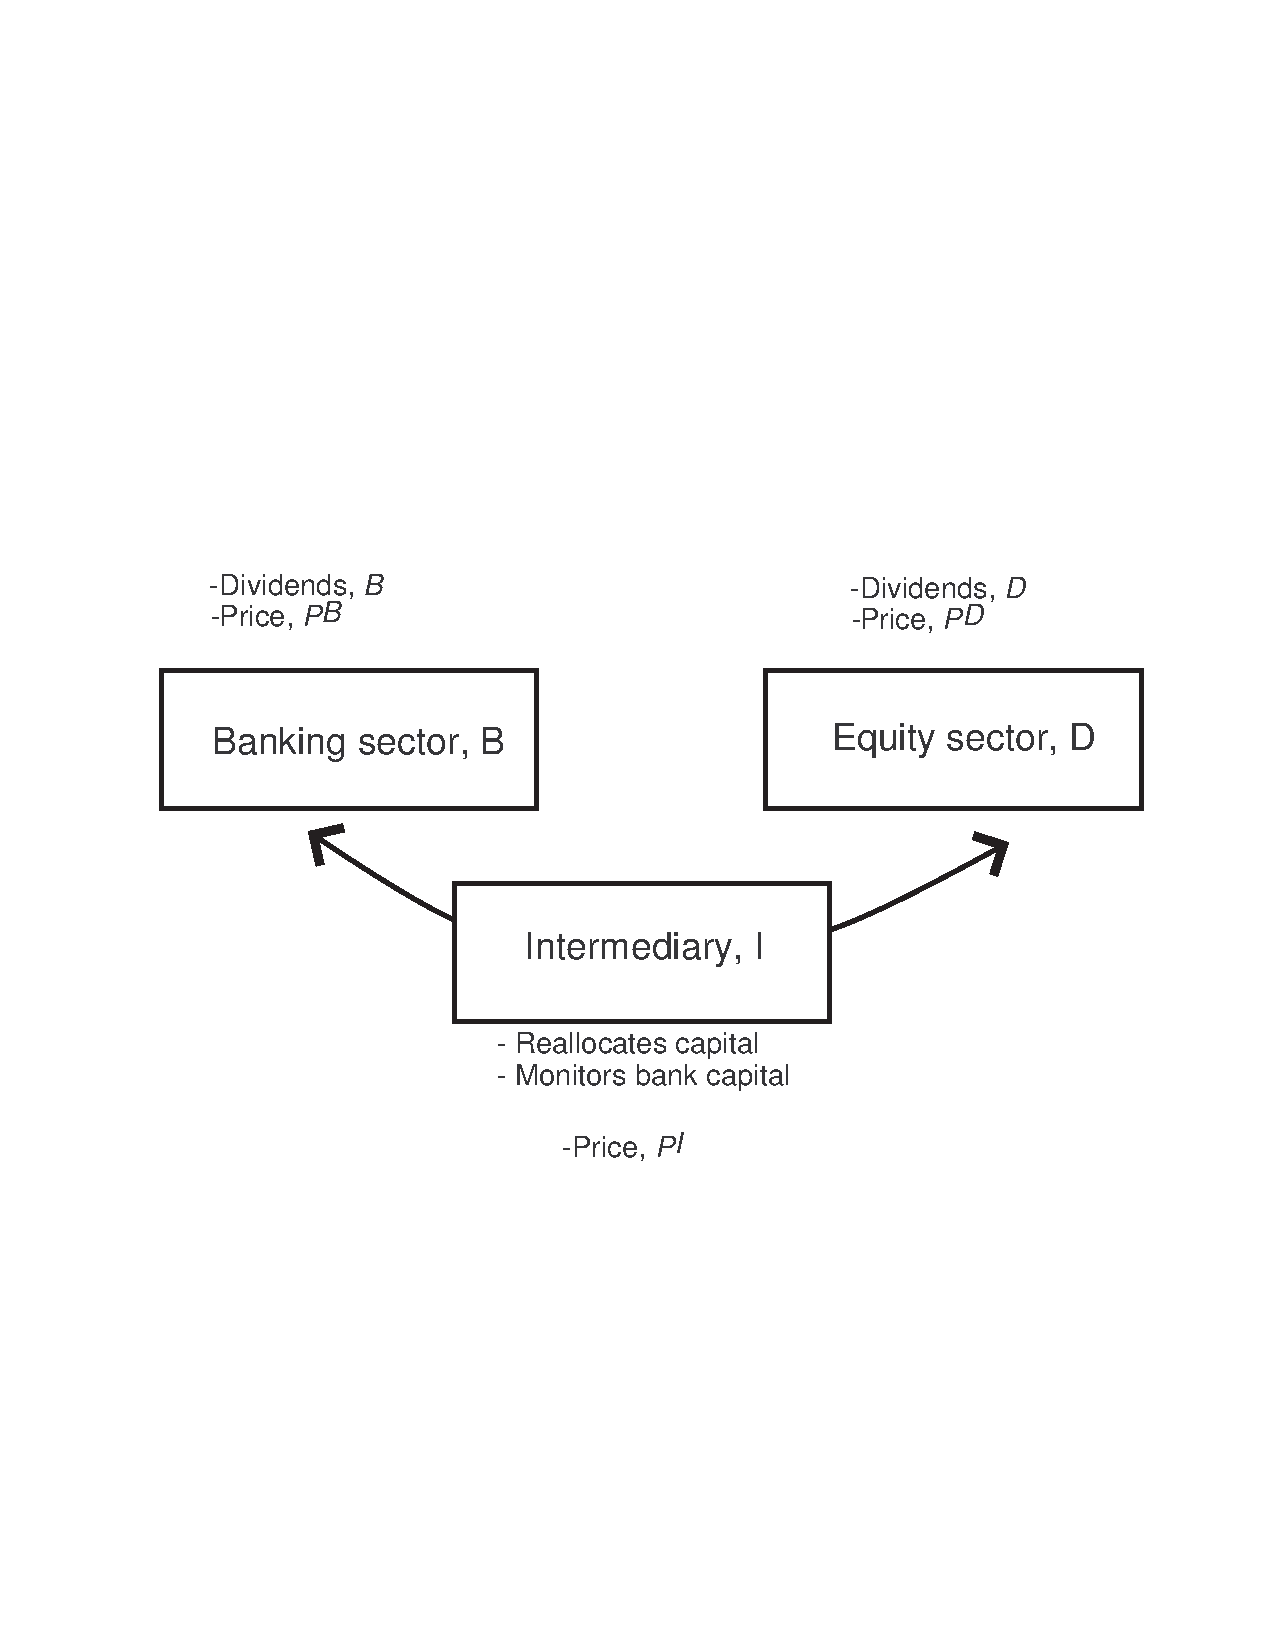
\includegraphics[width=7in]{Figure1}}
  \caption{{\bf Structure of model: capital can be invested in a bank sector and an equity sector.} An intermediary has the expertise to reallocate capital between the sectors and to monitor bank capital against bank crashes.} \label{fig:0}
\end{figure}
\vfill
\ 

\end{document}
